
\subsection{Replicated state machines}

\begin{center}
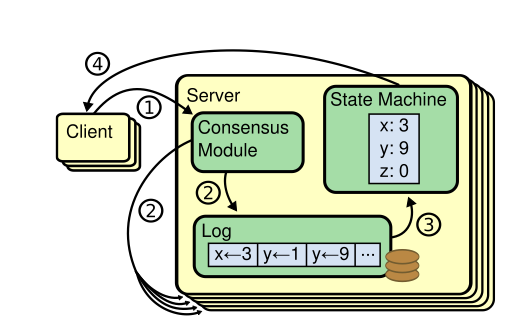
\includegraphics[scale=0.5]{img/repli_log}
\end{center}
\begin{itemize}
\item Consensus algorithm are used in the context of replicated state machines, used to solve a variety of fault tolerance problem in distributed systems.

\item Replicated state machines are typically implemented using a replicated log, as shown in Figure 1. Each server stores a log containing a series of commands, which its state machine executes in order. Each log contains the same commands in the same order, so each state ma- chine processes the same sequence of commands. Since the state machines are deterministic, each computes the same state and the same sequence of outputs.

\item Keeping the replicated log consistent is the job of the consensus algorithm. It ensures that every log will eventually contains the same requests in the same order. Each server's state machine processes the requests in log order and the outputs are returned to clients. The servers appear to form a single, highly reliable state machine. 

\item Consensus algorithms have the following properties :
\begin{itemize}
\item Safety : never return an incorrect result
\item Available : fully functional as long as a majority of the servers are operational and can communicate with each other and with clients.
\item Consistency : they don't depend on timing to ensure the consistency of the logs.
\item A command can complete as soon as a majority of the cluster has responded to a single round of remote procedure calls.
\end{itemize}

\end{itemize}

\subsection{Drawbacks of Paxos}

\begin{enumerate}
\item Difficult to understand.
\item Paxos doesn't provide a good foundation for building practical implementation.
\begin{itemize}
\item No widely agreed-upon algorithm for multi-Paxos (Combination of of multiple instances of single-decree Paxos to facilitate a series of decisions such as a log).
\item Paxos architecture is a poor one of building practical systems. This is a consequence of the single-decree decomposition.
\item Paxos uses a symmetric peer-to-peer approach as its core. This is not practical for system that need to made several decisions. It would be simpler and faster to first select a leader and then have the leader coordinates the decisions. 
\end{itemize}
\end{enumerate}

\subsection{Raft consensus algorithm}

\subsubsection{Basics}
\begin{itemize}

\item At any given time, each server is one of the three states : \textit{leader, follower, candidate}; 
\begin{itemize}
\item \textbf{Followers }: they issue no request on their own but simply respond to requests from leaders and candidates.
\item \textbf{Leader : } it handles all client requests.
\item \textbf{Candidate : } this state is used to elect a new leader.
\end{itemize}


\item Raft divides time into terms of arbitrary length. Each term begins with an election in order to have a new leader. If the election results in a split vote, there is no leader for this term and a new term with a new election will start shortly after. The terms act as logical clock, they allow servers to detect obsolete information. Each server stores a current term number. If one server's term is smaller then the other's then it updates its current term to the larger value. If a leader or a candidate discovers that its term is out of date, it immediately reverts to follower state. If a server receives a request with a stale term number, it rejects the request. Current term are exchanged when servers communicate with each other. 

\item Servers communicate with each other thanks to remote procedure calls. Especially, the \textbf{request vote} RPCs and the \textbf{append entries} RPCs. The first is initiated by candidates during the election and the second one by leader to replicate log entries and to provide a form of heartbeat. 

\end{itemize}

\subsubsection{Leader election}

\begin{itemize}

\item A server remains in the follower state as long as it receives heartbeat from the leader. If a follower receives no communication over the election timeout, it assumes there is no viable leader and begins an election. The election mechanism is the following :
\begin{enumerate}
\item A follower (the one who didn't receive heartbeat) increments its current term and transitions to candidate state. It then votes for itself and issues a \textbf{request vote} RPCs to the other servers.
\item Each server vote for at most one candidate in a given term, on a first-come-first-served basis. This can lead to two situations :
\begin{enumerate}
\item A candidate wins the election by receiving vote from a majority of servers. It then sends heartbeat to establish its authority.
\item Splite vote, and no leader for this term.
\end{enumerate}

\item To insure that the split vote situation doesn't happen again and again, Raft uses randomized election timeouts. Each candidate restarts its election timeout at the start of the election and it waits for that amount of time before starting the next election. By making this time random, the split vote situation is unlikely to happen often.
\end{enumerate}
\end{itemize}
\subsubsection{Log replication}

\begin{center}
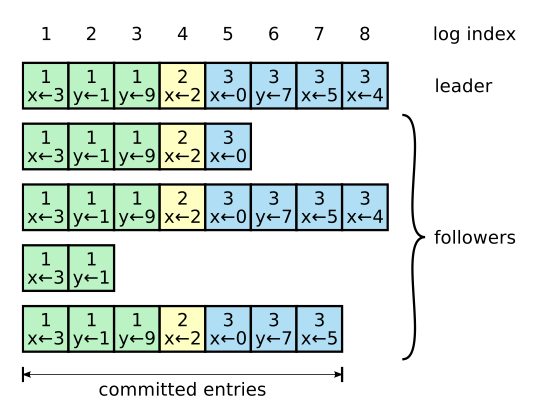
\includegraphics[scale=0.5]{img/logs}
\end{center}

\begin{itemize}


\item When communicating with the leader, clients send request with command to be executed by the replicated state machine. The leader appends the command to its log as a new entry and issued an \textbf{AppendEntries} RPCs to each servers to replicate the entry. The leader retries \textbf{AppendEntries} RPCs indefinitely until all followers eventually store all log entries, and applies the entry to its state machine and returns the result to the client. Raft guarantees that applied entries are durable and will eventually be executed by all of the available state machines. An entry is applied (committed) once the leader has replicated it on a majority of the servers. 


\item Log organization is shown on the figure. Each log entry has an integer to identify its position in the log and an integer with the term number when the entry was received. If two entries in different logs have the same index and term, then they store the same command and the logs are identical in all preceding entries. 

\item When issuing a \textbf{AppendEntries} for a new entry, the leader includes the index and term of the entry that precedes the new entry. If the follower doesn't find an entry in its log with the same index and term, it refuses the new entry and warns the leader that the entry was rejected. The leader maintains a \textit{nextIndex} for each follower which is the index of the next log entry the leader will send to that follower. When it receives a rejection, the leader decrements \textit{nextIndex} and retries the AppendEntries and such until the entry is accepted by the follower. Once the entry is accepted, the leader knows that the follower has the same log than its own ending at \textit{nextIndex}. It then forces the follower's log to duplicate its own starting at \textit{nextIndex}.

\end{itemize}

\subsubsection{Safety}

\paragraph*{Election restriction}
In order to ensure that the leader for any given term contains all of the entries committed in previous terms, Raft adds a restriction on which servers may be elected leader. Raft uses the voting process to prevent a candidate from winning an election unless its log contains all committed entries. If the candidate's log is at least as up-to-date as any other log in the majority, then if will hold all the committed entries and can be elected as leader. The \textbf{RequestVote} RPCs implements this restriction by including information about the candidate's log and the voter denies its vote if its own log is more up-to-date than that of the candidate. 

\paragraph{Timing and availability}
Leader election is the aspect of Raft where timing is most critical. Raft will be able to elect and maintain a steady leader as long as the system satisfies the following timing requirement : Broadcast Time $<<$ election Timeout $<<$ MTBF. Broadcast time is the average time for a server to send RPCs to every server in the cluster and receive their response; MTBF is the average time between failures for a single server. The broadcast time should be smaller than the election timeout so that leaders can reliably send the heartbeat to keep followers from starting elections. The election timeout should be less than MTBF so that the system makes steady progress. 

\subsection{Custer Membership changes}

In practice, it will be necessary to change the configuration (replace server, change degree of replication,...). Raft handles configuration changes without having to take the entire cluster off-line. To be safe, there must be no point during the transition where two leader can be elected for the same term. In order to achieve that goal, configuration changes must use a two-phase approach. First phase switches to a transitional configuration called joint consensus. Once the joint consensus has been committed, the system transitions to the new configuration. The joint consensus combines both the old and the new configuration : 
\begin{itemize}
\item All the log entries are replicated to all servers in both configuration
\item Any server from either configuration may serve as leader
\item Agreement requires separate majorities from \textit{both} the old and new configuration. 
\end{itemize}

Three more issues are still possible :

\begin{enumerate}
\item New servers in the configuration may not initially store any log entries (since they are new ones). The new servers join the cluster as non-voting members. The leader replicates log entries to them but they are not considered for majorities.
\item The cluster leader may not be part of the new configuration. The leader returns to the follower state once it has committed the log entries for the new configuration. There is then a time when the leader is managing a cluster that does not include itself; it replicates log entries but is not taken into account for majorities. 
\item Removed servers can disrupt the cluster. These servers will not re- ceive heartbeats, so they will time out and start new elec- tions. They will then send RequestVote RPCs with new term numbers, and this will cause the current leader to revert to follower state. A new leader will eventually be elected, but the removed servers will time out again and the process will repeat, resulting in poor availability. To prevent this problem, servers disregard RequestVote RPCs when they believe a current leader exists. This does not affect normal elections, where each server waits at least a minimum election timeout before starting an election. However, it helps avoid disruptions from re- moved servers: if a leader is able to get heartbeats to its cluster, then it will not be deposed by larger term numbers.
\end{enumerate}



